\documentclass[12pt]{scrartcl}
\usepackage[utf8]{inputenc}
\usepackage{amsmath,amssymb,amsthm}
\usepackage[croatian]{babel}
\usepackage{csquotes}
\MakeOuterQuote{"}
\usepackage{tikz}
\usetikzlibrary{positioning, fit, calc}
\usepackage[unicode]{hyperref}

% Za pisanje algoritama koji će oznaku `Algoritam` imati na hrvatskom jeziku koristim sljedeće pakete.
\usepackage{algorithm}
\usepackage[noend]{algpseudocode}
% izvor:
% https://tex.stackexchange.com/questions/230497/change-name-of-algorithm
\makeatletter
\newenvironment{algoritam}[1][htb]{%
    \renewcommand{\ALG@name}{Algoritam}% Update algorithm name
   \begin{algorithm}[#1]%
  }{\end{algorithm}}
\makeatother

\algrenewcommand\algorithmicfor{\textbf{Za sve}}
\algrenewcommand\algorithmicdo{\textbf{radi:}}
\algrenewcommand\algorithmicif{\textbf{Ako}}
\algrenewcommand\algorithmicthen{\textbf{onda:}}
\algrenewcommand\algorithmicreturn{\textbf{Vrati}}

\usepackage{subcaption}

\hypersetup{
    colorlinks,
    linkcolor={red!50!black},
    citecolor={blue!50!black},
    urlcolor={blue!80!black}
}

\usepackage[style=numeric]{biblatex}
\addbibresource{literatura.bib}

\usepackage{graphicx}
\usepackage{thmtools}

\declaretheorem{teorem}
\declaretheorem[sibling=teorem]{korolar}
\declaretheorem[name=Činjenica,sibling=teorem,qed=KRAJ]{cinjenica}
\declaretheorem[name=Tvrdnja,sibling=teorem]{tvrdnja}
\declaretheorem[style=definition,sibling=teorem,qed=$\vartriangleleft$]{definicija}
\declaretheorem[style=remark,qed=$\|$,sibling=teorem]{napomena}

\begin{document}

\title{Primjena Kruskalovog algoritma}  
\author{Mirna Imrović}
\date{Zagreb, \today}
\maketitle

\tableofcontents

\section{Uvod, glavni pojmovi}

U matematici i brojnim njenim primjenama svi smo se susreli s raznim vrstama algoritama. Ovisno o konkretnom problemu koji pokušavamo riješiti, \emph{pohlepni algoritmi} mogu biti jako korisni. 

\begin{definicija}\label{def:pohlepni}
\emph{Pohlepni algoritam} je algoritam koji u svakom svom koraku izabire lokalno najbolji izbor za nastavak, s ciljem dobivanja što boljeg ukupnog rješenja problema. 
\end{definicija}

Vrlo važan primjer pohlepnog algoritma je Kruskalov algoritam.

\begin{teorem}
Kruskalov algoritam za zadani graf $(V,E)$ generira minimalno razapinjuće stablo, odnosno podgraf grafa $(V,E)$ koji je ujedno i stablo, a suma duljina bridova je minimalna.
\end{teorem}

Ukratko, Kruskalov algoritam funkcionira tako da sortira bridove po duljini, traži komponentu povezanosti kojoj pripada neki vrh $x$ i spaja disjunktne komponente povezanosti. \emph{Pohlepnost} ovog algoritma proizlazi upravo iz traženja brida minimalne duljine koji će spojiti komponente povezanosti.

U ovom eseju prikazujemo primjenu Kruskalovog algoritma sa strukturom disjunktnih skupova na jednom jednostavnom problemu iz područja automatske analize programa.

\begin{definicija}\label{def:sds}
\cite{singer} \emph{Struktura diskjukntnih skupova} je apstraktna struktura podataka koja reprezentira particije nad danim skupom vrhova grafa. Nad ovom strukturom zadajemo sljedeće operacije:
\begin{itemize}
    \item \textsl{find}$(x)$ nalazi i vraća komponentu povezanosti kojoj pripada vrh $x$;
    \item \textsl{merge}$(A,B)$ spaja komponente povezanosti $A$ i $B$. \qedhere
\end{itemize}
\end{definicija}

\section{Iskaz konkretnog problema}

Neka su za skup varijabli $\{x_1,\dotsc,x_n\}$ zadani neki uvjeti oblika jednakosti, $x_i=x_j$, te neki uvjeti oblika nejednakosti, $x_i\neq x_j$. Je li moguće zadovoljiti sve uvjete?

Primjerice, za $n=4$ sljedeći skup uvjeta nije moguće zadovoljiti:

\begin{equation}\label{eq:npr}
    x_1=x_2,\quad x_2=x_3,\quad x_3=x_4,\quad x_1\neq x_4.
\end{equation}

Pronađimo efikasan algoritam s ulazom $m$ uvjeta i $n$ varijabli, koji odlučuje je li moguće zadovoljiti sve uvjete. 

Tekst problema preuzet je iz \cite{dasgupta}.

\section{Rješenje problema}

\subsection{Razrada ideje}

Pretpostavimo da želimo ručno riješiti ovaj problem za neku manju vrijednost broja $n$. Pokazuje se potreba da dane varijable na neki način skiciramo, kao i da naznačimo dane uvjete (ne)jednakosti. Skicirajmo skup uvjeta~\eqref{eq:npr}, koristeći zelene bridove za uvjete jednakosti, a crvene za uvjete nejednakosti:

\begin{center}
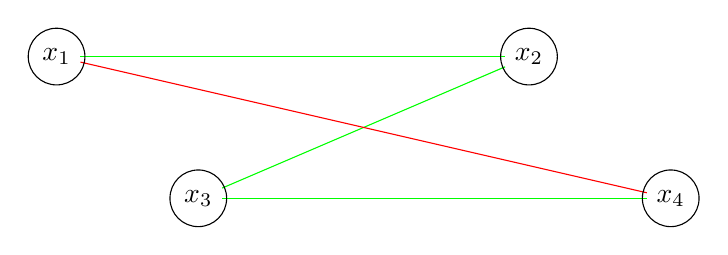
\begin{tikzpicture}[xscale = 6, yscale = 6]
\node (A) at (0,0.3) {$x_1$};
\node (B) at (1,0.3) {$x_2$};
\node (C) at (0.3,0) {$x_3$};
\node (D) at (1.3,0) {$x_4$};

\draw[green] (A) -- (B);
\draw[green] (B) -- (C);
\draw[green] (C) -- (D);
\draw[red]   (A) -- (D);

\draw (A) circle [radius = .06];
\draw (B) circle [radius = .06];
\draw (C) circle [radius = .06];
\draw (D) circle [radius = .06];
\end{tikzpicture}
\end{center}

Dakle, želimo problem svesti na dva podgrafa (sa zelenim i s crvenim bridovima) čiji su vrhovi naše varijable $x_1,...,x_n$, a jednakosti, odnosno nejednakosti, su bridovi. Ako postoje dva vrha koja su spojena u oba podgrafa, onda skup uvjeta nije moguće zadovoljiti.

\subsection{Formalizacija}
\begin{tvrdnja}
Neka je u nekom grafu skup vrhova dan s
\[V=\{x_1,...,x_n\},\]
skup bridova koji opisuju jednakosti dan s
\[E_1=\{\{x_i,x_j\} \mid x_i=x_j\}\]
i skup bridova koji opisuju nejednakosti dan s
\[E_2=\{\{x_i,x_j\} \mid x_i\neq x_j\}.\]
Tada su $(V,E_1)$ i $(V,E_2)$ ranije opisani podgrafovi, sa zelenim i crvenim bridovima, redom. 

Tvrdimo: ako postoje $i,j\in\{1,\dotsc,n\}$ takvi da u grafu $(V,E_1)$ postoji \emph{put} između $x_i$ i $x_j$, a u grafu $(V,E_2)$ postoji \emph{brid} između $x_i$ i $x_j$, onda skup uvjeta nije moguće zadovoljiti.
\end{tvrdnja}

\begin{proof}
Pretpostavimo da je problem rješiv. Ako postoji put od $x_i$ do $x_j$ u grafu $(V,E_1)$, zaključujemo da postoje neke varijable $x_{k_1},\dotsc,x_{k_l}$ t.d. vrijedi

\[x_i=x_{k_1},\quad x_{k_1}=x_{k_2}, \dotsc, x_{k_{l-1}}=x_l,\quad x_{k_l}=x_j.\]

Dakle, po tranzitivnosti vrijedi $x_i=x_j$, odnosno ne vrijedi i $x_i\neq x_j$ pa u grafu $(V,E_2)$ ne postoji brid između ta dva vrha.
\end{proof}

\section{Procedura}

Pri izradi algoritma koji će rješavati problem za $n$ čvorova i $m$ uvjeta koristimo se funkcijama \textsl{find} i \textsl{merge} iz definicije~\ref{def:sds}. Algoritam je sljedeći:

% "The algorithm environment is a float like table and figure" izvor: https://www.overleaf.com/learn/latex/Algorithms
\begin{algoritam}
\begin{algorithmic}\label{alg:zadovoljiv}
\For{$x_i\in V$}
    \State Načini skupove, odnosno disjunktne komponente povezanosti $\{x_i\}$
\EndFor
\For{$(x_i, x_j)\in E_1$}
    \State Uniraj komponente povezanosti koje sadrže $x_i$, $x_j$
\EndFor
\For{$(x_i, x_j)\in E_2$}
    \If{$x_i$ i $x_j$ pripadaju istoj komponenti povezanosti} 
        \Return NE
    \EndIf
\EndFor
\Return DA
\end{algorithmic}
\caption{Je li skup $m$ uvjeta nad $m$ varijabli zadovoljiv?}
\end{algoritam}

Prikažimo ideju postupka na jednostavnom primjeru. Neka je $n=5$ i uvjeti sljedeći:

\[
x_1 = x_2,\quad x_2 = x_3,\quad x_4 = x_5,\quad x_2 \neq x_5.
\]

Taj problem možemo skicirati na sljedeći način:

\begin{center}
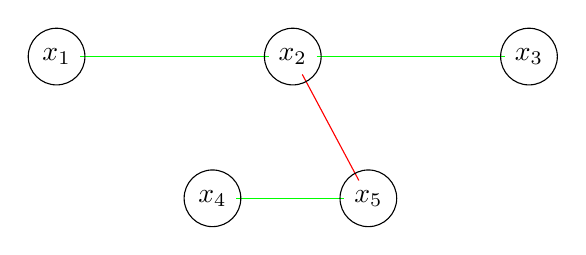
\begin{tikzpicture}[xscale=6, yscale=6]
\node (A) at (0,0.3) {$x_1$};
\node (B) at (0.5,0.3) {$x_2$};
\node (C) at (1,0.3) {$x_3$};
\node (D) at (0.33,0) {$x_4$};
\node (E) at (0.66,0) {$x_5$};

\draw[green] (A) -- (B);
\draw[green] (B) -- (C);
\draw[green] (D) -- (E);
\draw[red] (B) -- (E);

\draw (A) circle [radius = .06];
\draw (B) circle [radius = .06];
\draw (C) circle [radius = .06];
\draw (D) circle [radius = .06];
\draw (E) circle [radius = .06];
\end{tikzpicture}
\end{center}

Za dani graf postupak razdvajanja u disjunktne skupove je sljedeći:

% izvor za subfigure strukturu: https://tex.stackexchange.com/questions/120982/3-or-4-tikz-figures-side-by-side
\begin{figure}[!h]
    \centering
    \begin{subfigure}[t]{0.45\textwidth}
        \centering
        \resizebox{\linewidth}{!}{
            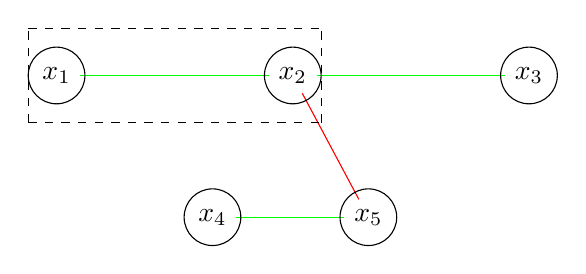
\begin{tikzpicture}[xscale=6, yscale=6]
                \node (A) at (0,0.3) {$x_1$};
                \node (B) at (0.5,0.3) {$x_2$};
                \node (C) at (1,0.3) {$x_3$};
                \node (D) at (0.33,0) {$x_4$};
                \node (E) at (0.66,0) {$x_5$};
                
                \draw[green] (A) -- (B);
                \draw[green] (B) -- (C);
                \draw[green] (D) -- (E);
                \draw[red]   (B) -- (E);
                
                \draw (A) circle [radius = .06];
                \draw (B) circle [radius = .06];
                \draw (C) circle [radius = .06];
                \draw (D) circle [radius = .06];
                \draw (E) circle [radius = .06];
            
                % pravokutnik oko x1, x2
                \draw[dashed] (-0.06,0.4) -- (0.56,0.4);
                \draw[dashed] (-0.06,0.2) -- (0.56,0.2);
                \draw[dashed] (-0.06,0.2) -- (-0.06,0.4);
                \draw[dashed] (0.56,0.2) -- (0.56,0.4);
            \end{tikzpicture}
        }  
        \caption{Prvi brid tipa jednakosti}
        \label{fig:A}
    \end{subfigure}
    \begin{subfigure}[t]{0.45\textwidth}
        \centering
        \resizebox{\linewidth}{!}{
            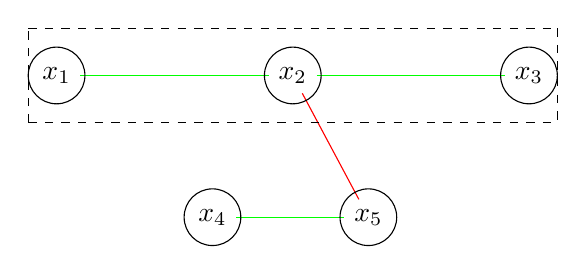
\begin{tikzpicture}[xscale=6, yscale=6]
                \node (A) at (0,0.3) {$x_1$};
                \node (B) at (0.5,0.3) {$x_2$};
                \node (C) at (1,0.3) {$x_3$};
                \node (D) at (0.33,0) {$x_4$};
                \node (E) at (0.66,0) {$x_5$};
                
                \draw[green] (A) -- (B);
                \draw[green] (B) -- (C);
                \draw[green] (D) -- (E);
                \draw[red]   (B) -- (E);
                
                \draw (A) circle [radius = .06];
                \draw (B) circle [radius = .06];
                \draw (C) circle [radius = .06];
                \draw (D) circle [radius = .06];
                \draw (E) circle [radius = .06];
            
                % pravokutnik oko x1, x2, x3
                \draw[dashed] (-0.06,0.4) -- (1.06,0.4);
                \draw[dashed] (-0.06,0.2) -- (1.06,0.2);
                \draw[dashed] (-0.06,0.2) -- (-0.06,0.4);
                \draw[dashed] (1.06,0.4) -- (1.06,0.2);
            \end{tikzpicture}
        }
        \caption{Drugi brid tipa jednakosti pripada istoj komponenti povezanosti}
        \label{fig:B}
    \end{subfigure}
    \begin{subfigure}[b]{0.45\textwidth}
        \centering
        \resizebox{\linewidth}{!}{
            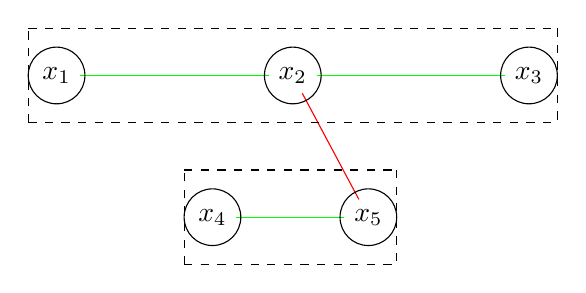
\begin{tikzpicture}[xscale=6, yscale=6]
                \node (A) at (0,0.3) {$x_1$};
                \node (B) at (0.5,0.3) {$x_2$};
                \node (C) at (1,0.3) {$x_3$};
                \node (D) at (0.33,0) {$x_4$};
                \node (E) at (0.66,0) {$x_5$};
                
                \draw[green] (A) -- (B);
                \draw[green] (B) -- (C);
                \draw[green] (D) -- (E);
                \draw[red]   (B) -- (E);
                
                \draw (A) circle [radius = .06];
                \draw (B) circle [radius = .06];
                \draw (C) circle [radius = .06];
                \draw (D) circle [radius = .06];
                \draw (E) circle [radius = .06];
            
                % pravokutnik oko x1, x2, x3
                \draw[dashed] (-0.06,0.4) -- (1.06,0.4);
                \draw[dashed] (-0.06,0.2) -- (1.06,0.2);
                \draw[dashed] (-0.06,0.2) -- (-0.06,0.4);
                \draw[dashed] (1.06,0.4) -- (1.06,0.2);
                
                % pravokutnik oko x4, x5
                \draw[dashed] (0.27, -0.1) -- (0.72, -0.1);
                \draw[dashed] (0.27, 0.1) -- (0.72, 0.1);
                \draw[dashed] (0.27, -0.1) -- (0.27, 0.1);
                \draw[dashed] (0.72, 0.1) -- (0.72, -0.1);
            \end{tikzpicture}
        }
        \caption{Dodamo i treći brid tipa jednakosti}
        \label{fig:C}
    \end{subfigure}
    \caption{Provođenje algoritma \ref{alg:zadovoljiv}}
\end{figure}

Uočimo kako jedini crveni brid na slici \ref{fig:C} spaja čvorove koji ne pripadaju istim komponentama povezanosti, što znači da je problem rješiv. Međutim, kad bi bio dodan još i uvjet $x_1\neq x_3$, problem bi prestao biti rješiv!

\section{Implementacija}

Za implementaciju ovog algoritma pretpostavljamo da imamo implementirane metode \verb`find` i \verb`merge` iz definicije~\ref{def:sds}. (Za implementaciju vidi \cite{singer}.) Pritom \verb`find` vraća oznaku skupa kojem pripada dani argument. 

Čvor varijable $x_i$ bit će reprezentiran cijelim brojem \verb`i-1`.

Dodatno, koristimo sljedeća polja:
\begin{itemize}
    \item \verb`skup[]` na $i$-tom indeksu ima najmanji indeks čvora koji pripada istoj komponenti povezanosti;
    \item \verb`E1[][]` predstavlja parove čvorova koji su međusobno jednaki (zeleni bridovi);
    \item \verb`E2[][]` predstavlja parove čvorova koji su međusobno različiti (crveni bridovi).
\end{itemize}

Preformulirajmo algoritam~\ref{alg:zadovoljiv} u terminima gore navedenih metoda i polja:

\begin{verbatim}
    bool problemZadovoljiv() {
        for(int i = 0; i <= n; i++) {
            skup[i] = i;
        }
        for(int i = 0; i <= n; i++) {
            for(int j = 0; j <= n; j++) {
                if(E1[i][j] == 1) merge(i, j);
            }
        }
        for(int i = 0; i <= n; i++) {
            for(int j = 0; j <= n; j++) {
                if(E2[i][j] == 1 && find(i) == find(j)) return false;
            }
        }
        return true;
    }    
\end{verbatim}

\section{Složenost}
Konačno, potrebno je izračunati ukupnu složenost sastavljenog algoritma. 
\begin{itemize}
    \item Inicijalizacija skupova mora proći kroz sve čvorove pa je složenosti $O(n)$.
    \item Na svakom bridu iz skupa $E_1$ poziva se metoda \verb`merge`, za koju se može pokazati da je složenosti $O(\log^*(n))$. Stoga drugi korak algoritma ima složenost $O(|E_1|\cdot\log^*(n))$.
    \item Slično, na svakom bridu iz $E_2$ poziva se \verb+find+, pa je složenost trećeg koraka algoritma $O(|E_2|\cdot\log^*(n))$.
\end{itemize}

Pritom je 
$$\log^*(n) = \underbrace{\log(\log(...(\log}_\text{$k$ puta}(n)))), $$
gdje je $k$ najmanji prirodni broj za koji vrijedi da je $\log^*(n)\le1$. Slijedi da je ukupna složenost algoritma
\[O(n+m\cdot\log^*(n)). \]

\printbibliography

\end{document}
